\documentclass[11pt,twoside]{report} 
\usepackage[utf8]{inputenc}

\usepackage{geometry} % to change the page dimensions
\geometry{a4paper}
\usepackage{url}
\usepackage{graphicx} 
\usepackage{booktabs} 
\usepackage{array} 
\usepackage{paralist} 
\usepackage{verbatim} 
\usepackage{subfig} 
\usepackage{amsmath}
\usepackage{fancyhdr} 
\pagestyle{fancy} 
\renewcommand{\headrulewidth}{0pt} 
\lhead{}\chead{}\rhead{}
\lfoot{}\cfoot{\thepage}\rfoot{}
\usepackage{fullpage}
\usepackage[active]{srcltx}

\usepackage{sectsty}
\allsectionsfont{\sffamily\mdseries\upshape}


\usepackage[nottoc,notlof,notlot]{tocbibind} 
\usepackage[titles,subfigure]{tocloft} 
\renewcommand{\cftsecfont}{\rmfamily\mdseries\upshape}
\renewcommand{\cftsecpagefont}{\rmfamily\mdseries\upshape} 



\title{Groundwater Contamination}
\author{Ivan Marin}
\date{\today} 

\begin{document}
\maketitle
\tableofcontents

%=================================================================================================
\chapter{Groundwater Contamination}
\section{Groundwater Contamination}
Groundwater contamination can start with the spill of contaminant liquids, or the dissolution of contaminants in water in the surface. Several processes (chemical, physical and biological) occur in the transit of the contaminant from the surface to the subsurface and in the subsurface, being able to reduce the concentration of the contaminant. 

But even low concentrations of the contaminants can be toxic to human life. Remediation, the process of cleaning up or removing the contaminants from the subsurface can be very expensive, when it's possible. 

\subsection{Sources of Contamination}
The sources of anthropogenic contamination are 
\begin{itemize}
 \item Agriculture,
 \item Industrial activities,
 \item Domestic activities
 \item and contamination sources like storage tanks, pipes, evaporation or stabilization ponds, aerobic, anaerobic and facultative lagoons.
\end{itemize}

Another process of groundwater contamination is the precipitation of compounds in suspension in the atmosphere by rain. Runoff can also dissolve compounds in the surface, generating contamination of surface water bodies or infiltration and subsequent subsurface contamination. 


\subsection{Types of Contaminants}
The contaminants can be \textit{organic} or \textit{inorganic}:
Some organic contaminants:
\begin{itemize}
 \item Detergents
 \item chlorinated hydrocarbons: chloroform, carbon tetrachloride, trichloroethylene, PCB (DNAPLs)
 \item aromatic hydrocarbons: benzene, naphthalene (LNAPLs)
 \item Petroleum hydrocarbons, like gasoline, diesel, lubricants (LNAPLs)
 \item volatile organic compounds, like solvents
 \item pesticides, organochlorines, organophosphates and carbamates
\end{itemize}


Some inorganic contaminants:

\begin{itemize}
   \item Acidity from industrial contaminants
   \item Ammonia $NH_{3}$
   \item Fertilizers: $NO_{3}^{-2}$, $PO_{4}^{-3}$
   \item Heavy Metals: $Fe, As, Cd, Mg, Hg, Pb$
   \item Nuclear Waste from NPP\footnote{Nuclear Power Plants} and mining operations
   \item Acid deposition (acid rain)
   \item Thermal Pollution 
\end{itemize}

Other types of contaminants are pathogenic bacteria and viruses. 

\subsubsection{Heavy Metals}
Defined by high thermal and electrical conductivity, high reflectivity, ductility and strength. Form cations on solutions. Heavy metals are metals with specific weight greater than 4.0 $g/cm^{3}$. Usually are Hg, Pb, Cd, As, B, Al, Cr, Bs, Co, Ni, St, Zn, Ti. Metals are persistent, only being removed by groundwater movement, adsorbed or precipitated. Sources: mining, landfills. 

\subsubsection{Organic Contaminants}
Organic molecules are composed by a carbon atom structure, connected by covalent bounds and other chemical elements. The most common chemical elements besides carbon are H, O, N, S, F, Cl, Br, I. There are usually formed in living organisms. The organic molecules can be aliphatic, when the carbons are layout as a line, or aromatic, when connected in a ring form. 

Groundwater usually has lower concentrations of organic compounds known as humic substances, originated by decomposition of organic materiél by microorganisms near the surface. The humic substances are usually divided in two categories: humic acids, soluble in water, and fulvic acids. 

The quantification of the dissolved organic carbon (DOC) is measured oxidizing all organic materials present in the water into CO2 and quantifying the gas. DOC concentrations usually have a descending gradient with depth. 

\subsubsection{Pathogens}
Pathogens can be bacteria, virus, protozoa and helminths (worms). Their relation with diseases are variate: They can caused by drinking the contaminated water (cholera), related with the lack of water to hygiene (trachoma), transmitted by the contact with water without ingestion (schistosomiasis) and water being a host for the proliferation (dengue).

\subsubsection{Oxygen Consuming Waste}
Oxygen concentration in water can be reduced by biodegradation, when oxygen is consumed when the organic compounds are used. 

\subsubsection{Salts}
Salts and total dissolved solids sources are usually application of road salts and irrigation.

\subsubsection{Acid Deposition}
Rain water usually has pH about 5.7, but anthropogenic emissions can lower to pH around 4, mostly because of the $H^{+}$, $NO_{3}^{-}$ and $SO_{4}^{2-}$. Rain with water more acidic can dissolve harmful components in the soil.

\subsection{NAPLs}
\textit{NAPL} (Non-Aqueous Phase Liquids) is a very broad category for organic compounds that form a distinct phase from the aqueous one. They have a very low solubility in water\footnote{The groundwater texts usually refers to NAPLs as \textit{immiscible} because of its low solubility, but this term can cause confusion, as all liquids are miscible in water, with different solubilities.}. NAPLs are a great concern for groundwater contamination as even very low concentrations (less than ppb in some cases) are above the recommended levels for human water consumption. Also the general name NAPL is used for single compounds, like TCE, and mixtures of several NAPLs, like gasoline. This is relevant when dissolution of the NAPL has to be taken into account. 

\textit{LNAPLs} are called \textit{Light} because they have a lower density than water, and \textit{DNAPLs} are \textit{Dense} for the inverse reason, with densities higher than water. 

\textit{BTEX}, Benzene, Toluene, Ethylbenzene and Xylene forms a LNAPL. The chlorinated components like  
tetrachloroethylene (PCE), trichloroethylene (TCE), 1,2-dichloroethylene (DCE), 1,2-dichloroethane (DCA),  vinylchloride (VC) and carbon tetrachloride (CTC). These compounds have higher specific weight than that of water and form a DNAPL.

\section{Geometric Source Classification}
Another form of source classification is a geometric one. Sources can be point or distributed (also called difused sources). The geometric classification must take into account the domain of interest: a point source for one domain can be a distributed one for another domain considered. 

A \textit{Point Source} has a very small spacial distribution, while a \textit{Distributed Source} has a large horizontal extension, considering the domain of interest. Some examples of point sources:

\begin{itemize}
   \item septic tanks,
   \item industrial discharges,
   \item sewage discharges,
   \item storage tank and pipeline leaks,
   \item transport accidents,
   \item abandoned wells,
   \item landfills, 
   \item aerobic and anaerobic ponds
\end{itemize}

It's important to note again that some of these sources can be considered distributed sources depending on the scale of the domain of interest.

Some examples of distributed sources are
\begin{itemize}
   \item application of herbicides and pesticides
   \item application of fertilizers
   \item animal herding
   \item irrigation
\end{itemize}

\textit{Landfills} can produce leachate, depending on the conditions of the waste, the percolation speed and the waste age. 

The combination of fertilizers, pesticides and irrigation, common in an agricultural setting, can generate serious contamination problems. 

\section{Geochemistry of (L/D)NAPLs}
NAPLs introduced by spills first have to percolate through the unsaturated zone, where a multiphase system composed by air, water and the NAPL is formed. The vapours generated by the evaporation of the NAPL in the vadose zone can generate also a gaseous NAPL phase, that can then be transported for long distances in the subsurface. 

NAPLs usually have low solubilities in water, creating a sharp interface between the different phases (air-NAPL, water-NAPL). For example, the solubility of TCE in water at 20 C is $1,1 \times 10^{6}$. Depending on the size of the pores and the presence of zones with lower permeability, like clay lenses, percolation can generate lateral spreading, leaving regions with disconnected droplets trapped in pore space, being immobile with usual hydraulic gradients. Three zones for the NAPL can be formed: a dissolved one, being transported by the groundwater; a residual zone, with the DNAPL trapped in the pores, disconnected and not moving with the hydraulic gradient, and pools - large concentrations - of the liquid. 


The behavior of the LNAPL and DNAPL are different when they reach the phreatic surface. The difference in density is the responsible for this.

\begin{figure}
   \centering
   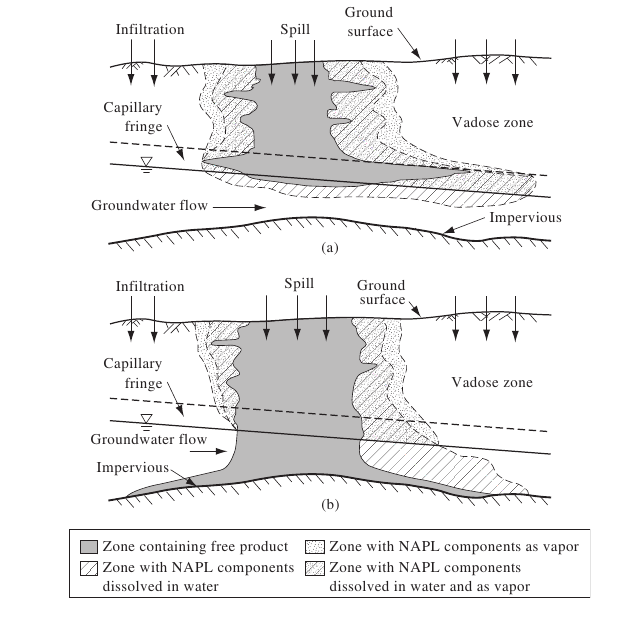
\includegraphics[width=8cm]{./img/bear-ldnapl.png}
   % bear-ldnapl.png: 617x617 pixel, 72dpi, 21.76x21.76 cm, bb=0 0 617 617
   \label{ldnapl}
   \caption{Representation of a large spill of (L/N)NAPL. From \cite{bearcontaminant}}
\end{figure}

The residual zone is composed by NAPL in a \textit{residual phase}, when the NAPL reach a saturation where it cannot overcome the partial pore pressure and is not able to move with the hydraulic gradient. 

The processes involved in NAPL in groundwater are
\begin{itemize}
   \item Volatilization (Henry's Law)
   \item Dissolution
   \item Sorption
   \item Biodegradation
\end{itemize}

\bibliographystyle{plain}
\bibliography{bibliografia/bibliografia}

\end{document}

